Organize this section according to the rules defined in the project description. 

\subsection{External Interface Requirements}
\subsubsection{User interfaces}
The user interface will be responsive and should be multiple platform. Even if it should be mainly done for phones. \newline

Where as the application for policy makers should be also responsive but mainly optimized for computer.



First we will present the interfaces for farmers. They are not exhaustive but the goal here is to give a good overview of what the app will look like. The figure \ref{Fig:interface_login} represents the general login page. Depending on the mail the user will then be a farmer or a policy maker.

\begin{figure}[H]

	\centering

	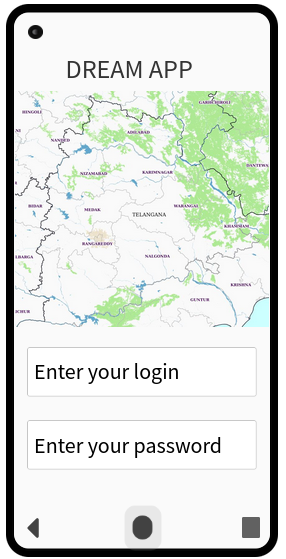
\includegraphics[width=0.2\columnwidth]{Images/login.png}

	\caption{login from a phone}

	\label{Fig:interface_login}

\end{figure}



The figure \ref{Fig:interface_forum} shows the view of the forum on a phone, this view as the others will also be visible from a computer as all the app will be responsive. Next to it the figure \ref{Fig:interface_meteo} gives access to the main data simply and in a rapid way.

\begin{figure}[H]

	\begin{minipage}{0.48\textwidth}

		\centering

		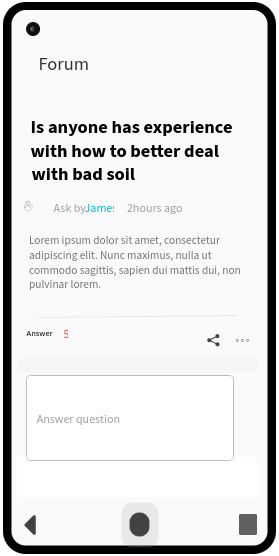
\includegraphics[width=0.6\columnwidth]{Images/forum.png}

		\caption{forum from a phone}

		\label{Fig:interface_forum}

	\end{minipage}

	\begin{minipage}{0.48\textwidth}

		\centering

		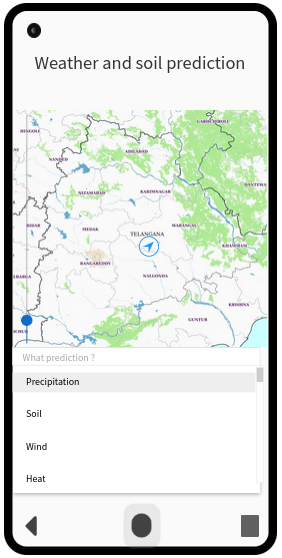
\includegraphics[width=0.6\columnwidth]{Images/meteo.png}


The communication interfaces of the different sensors is external.




		\caption{have access to data}

		\label{Fig:interface_meteo}

	\end{minipage}\hfill

\end{figure}

\begin{figure}[H]

	\centering

	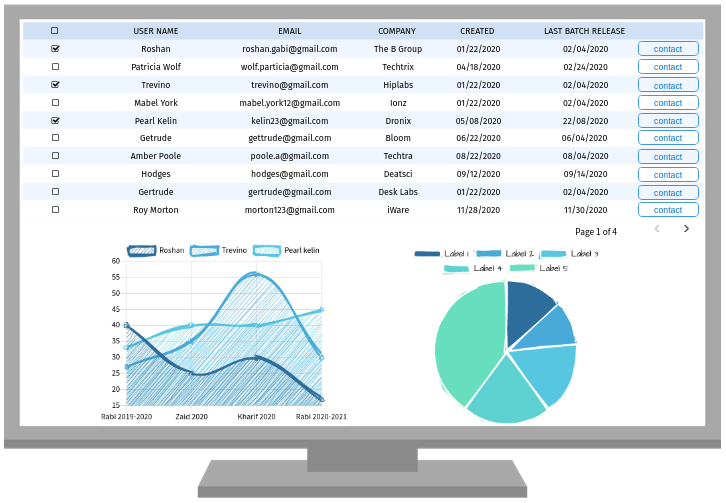
\includegraphics[width=0.8\columnwidth]{Images/visualize_farmers.png}

	\caption{Policy Maker comparing farmer on different factors}

	\label{Fig:interface_visu_farmers}

\end{figure}



\begin{figure}[H]

	\centering

	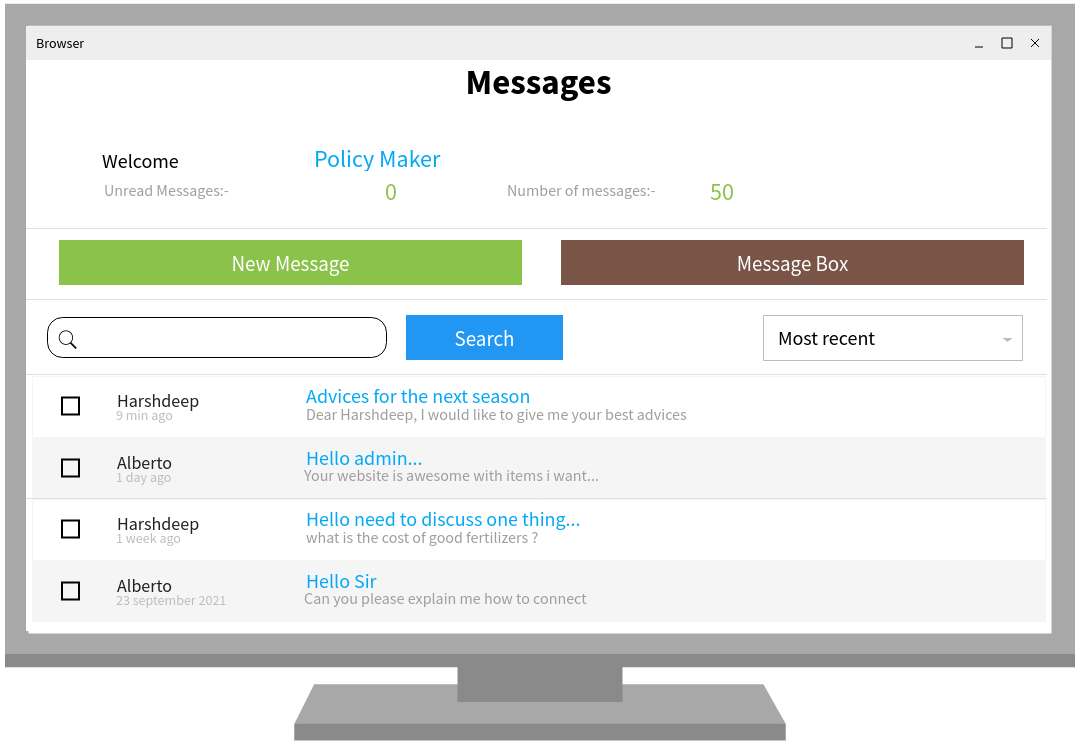
\includegraphics[width=0.8\columnwidth]{Images/messages_policy_maker.png}

	\caption{Policy Maker messages}

	\label{Fig:interface_messages_policy_maker}

\end{figure}

\subsubsection{Hardware Interfaces}
\subsubsection{Software Interfaces}
\subsubsection{Communication Interfaces}
\subsection{Functional requirements}
% Definition  of  use  case  diagrams,  use  cases  and  associated sequence/activity diagrams, and mapping on requirements 
\begin{table}[htbp]
	\centering
	\begin{tabularx}{\linewidth}{|l|X|}
		\hline
		Name & \multicolumn{1}{c|}{\textit{\textbf{FarmerRegistration}}}                                                   \tabularnewline \hline
		Actors                                               & Farmers                                                    \tabularnewline \hline
		Entry conditions                                              & The farmer is on the DREAM registration form page                                                                                  \tabularnewline \hline
		Event flow                                         & 1.	The system asks for farmer’s data: name, surname, e-mail address, location.                                                                    \tabularnewline 
		& 2.	The farmers fill out the form. The farmer can optionally enable geo-tracking to complete the location field.                                                   \tabularnewline 
		& 3.	The farmer confirms the responses.                                                   \tabularnewline 
		& 4.	The system sends an e-mail containing a validation link to the given e-mail address.                                                \tabularnewline
		& 5.	The system asks the farmer to check his/her e-mail box.                                               \tabularnewline
		& 6.	The farmer clicks on the validation link.                                     \tabularnewline
		& 7.	The system adds the data provided by the farmer to the database.                                  \tabularnewline
		& 8.	Based on the location given by the farmer, the system retrieves the e-mail address of the policy maker dedicated to the farmer newly registered.                               \tabularnewline
		& 9.	The system sends an e-mail to the policy maker to acknowledge that a new farmer has registered.                              \tabularnewline \hline
		Exit conditions & The data are correctly added to the database
		\tabularnewline \hline
		Exceptions & 
		-	The given e-mail address is already in the database. The system displays a message prompting the farmer to modify the dedicated field of the form.  \tabularnewline
		
		&-	The data provided by the farmer have an invalid type or the e-mail address is incorrect. The system displays a message prompting the farmer to modify the dedicated field(s) of the form. 
		\tabularnewline
		&-	There is no registered policy maker dedicated to the area. In that case, no acknowledgement e-mail is sent, but instead a warning message is sent to the developer to urge him/her to contact the adequate policy maker. 
		\tabularnewline
		\hline
	\end{tabularx}   
\end{table}

\begin{table}[htbp]
	\centering
	\begin{tabularx}{\linewidth}{|l|X|}
		\hline
		Name & \multicolumn{1}{c|}{\textit{\textbf{ProductionRelease}}}                                                   \tabularnewline \hline
		Actors                                               & Farmers                                                    \tabularnewline \hline
		Entry conditions                                              & The farmer has begun the cropping season (and eventually finished). \tabularnewline
		&The farmer is already registered on the DREAM platform
		\tabularnewline \hline
		Event flow                                         & 1.	The farmer logs in on the platform and clicks on the “Release production data” tab.                                                                   \tabularnewline 
		& 2.	The farmer clicks on the “New release” button                                                   \tabularnewline 
		& 3.	The system displays a form with the following fields: seed variety (to be chosen among a certain list), seed rate, production amount, surface area of the cultivated fields, fertilizer (can be several, to be chosen among a certain list), amount of fertilizer used (one field per fertilizer used), start and end date.                                                 \tabularnewline 
		& 4.	The farmer completes the fields, with respect to the measure units given by the system.                                           \tabularnewline
		& 5.	The farmer confirms.                                               \tabularnewline
		& 6.	The system adds the data to the database with the status "Complete".      
		\tabularnewline \hline
		Exit conditions 
		& 
		The data are correctly added to the database
		\tabularnewline \hline
		Exceptions 
		& 
		-	The data provided by the farmer have an invalid type. The system displays a message prompting the farmer to modify the dedicated field(s) of the form
		\tabularnewline
		&-	All the data are not provided (e.g. the end date, the production amount) because cropping has not ended yet. The data are added to the database with an “Incomplete” status. If seed variety, seed rate, surface area or start date are not provided, the system displays an error message
		\tabularnewline
		\hline
	\end{tabularx}   
\end{table}

\begin{table}[htbp]
	\centering
	\begin{tabularx}{\linewidth}{|l|X|}
		\hline
		Name & \multicolumn{1}{c|}{\textit{\textbf{ForumCreation}}}                                                   \tabularnewline \hline
		Actors                                               & Farmers                                                    \tabularnewline \hline
		Entry conditions                                              &
		The farmer is already registered on the DREAM platform
		\tabularnewline
		Event flow                                         & 1.	The farmer logs in on the platform and clicks on the “Forum” tab.                                           \tabularnewline 
		& 2.	The farmer clicks on the “New topic” button.                                            \tabularnewline 
		& 3.	The farmer completes the title and message fields                                            \tabularnewline 
		& 4.	The farmer can optionally add some tags to characterize the topic                                    
		\tabularnewline 
		&
		5.	The system adds the topic to the database
		\tabularnewline \hline
		Exit conditions 
		&  The data are correctly added to the database
		\tabularnewline \hline
		Exceptions 
		& 
		-	The data provided by the farmer have an invalid type. The system displays a message prompting the farmer to modify the dedicated field(s) of the form.
		\tabularnewline
		&-	The title or the message is empty. The system displays a message prompting the farmer to fill them both.
		\tabularnewline
		\hline
	\end{tabularx}   
\end{table}

\begin{table}[htbp]
	\centering
	\begin{tabularx}{\linewidth}{|l|X|}
		\hline
		Name & \multicolumn{1}{c|}{\textit{\textbf{PredictionCheck}}}                                                   \tabularnewline \hline
		Actors                                               & Farmers                                                    \tabularnewline \hline
		Entry conditions                                              &
		The farmer is already registered on the DREAM platform
		\tabularnewline
		&
		\tabularnewline \hline
		Event flow                                         & 1.	The farmer logs in on the platform                                         \tabularnewline 
		& 2.	From the homepage, the farmer clicks on the desired button, between “soil”, “weather” and “vegetation index”.                                          \tabularnewline 
		& 3.	Based on the location of the farmer, the system displays a map for the conditions (and eventually another one for the predictions), with the time period.                                           \tabularnewline 
		& 4.	The farmer can optionally zoom in/out and move on the map provided by the system.                                    \tabularnewline \hline
		Exit conditions 
		& The farmer leaves the homepage
		\tabularnewline \hline
		Exceptions 
		& -	There is no data corresponding to the current time or the location of the farmer. In the first case, the system proposes to display results for a close time (if it exists). In the second case, it zooms out until finding a place where data are available (if they exist)
		\tabularnewline
		\hline
	\end{tabularx}   
\end{table}

\begin{table}[htbp]
	\centering
	\begin{tabularx}{\linewidth}{|l|X|}
		\hline
		Name & \multicolumn{1}{c|}{\textit{\textbf{RequestForProductionData}}}                                                   \tabularnewline \hline
		Actors                                               & Farmers                                                    \tabularnewline \hline
		Entry conditions                                        
		& The farmer is already registered on the DREAM platform and has not confirmed the data for the last cropping season.
		\tabularnewline
		&
		The current date is in a 15 days-range before the end of a cropping season (15/11-01/12, 15/04-01/5 or 15/07-01/08).
		\tabularnewline \hline
		Event flow                                         & 1.	The system sends an e-mail to recall the farmer to release the production data                                           \tabularnewline 
		& 2.	The farmer logs in on the platform.                                             \tabularnewline 
		& 3.	The system displays a notification with a link to the “Release production data” tab.                                           \tabularnewline 
		& 4.	The farmer clicks on the link.                                    \tabularnewline
		& 5.	The system displays the “Release production data” tab, with an additional “Confirm the data for this season” button.                                           \tabularnewline
		& 6.	The farmer eventually creates a new release or completes the releases with an "Incomplete" (see ProductionRelease use case).                                     \tabularnewline
		& 7.	Within 15 days, the farmer clicks on the button “Confirm the data for this season”                                \tabularnewline
		& 8.	The system adds the farmer to the list of farmers who confirmed their release for the season                              \tabularnewline
		& 9.	The system hides the button “Confirm the data for this season”                       \tabularnewline \hline
		Exit conditions 
		& The system adds the farmer to the list of farmers who completed their release 
		\tabularnewline \hline
		Exceptions 
		& 
		-	The farmer does not click on the button “Confirm the data for this season”. At every log in, the system will display the notification to release the data production
		\tabularnewline
		&
		-	The farmer adds or modifies a production data release after having clicked on the button “Confirm the data for this season”. The system removes the farmer from the list of farmers who completed their release for the season. The system displays the button “Confirm the data for this season” again
		\tabularnewline
		\hline
	\end{tabularx}   
\end{table}

\begin{table}[htbp]
	\centering
	\begin{tabularx}{\linewidth}{|l|X|}
		\hline
		Name & \multicolumn{1}{c|}{\textit{\textbf{TopicResearch}}}                                                   \tabularnewline \hline
		Actors                                               & Farmer, Policy Maker                                                   \tabularnewline \hline
		Entry conditions                                              & The actor is already registered on the DREAM platform
		\tabularnewline
		&
		\tabularnewline \hline
		Event flow                                         & 1.	The actor logs in on the platform and clicks on the “Forum” tab.                                           \tabularnewline 
		& 2.	The actor clicks on the “Search” button.                                           \tabularnewline 
		& 3.	The system displays a search bar and two optional filters: date and tags.                                           \tabularnewline 
		& 4.	The actor completes the field and eventually add some filters.                                    \tabularnewline
		& 5.	The actor confirms the request.                                           \tabularnewline
		& 6.	The system fetches and displays the list of results.                                     \tabularnewline
		& 7.	The actor clicks on one of them.                                \tabularnewline
		& 8.	The system displays the discussion thread on the topic.                              \tabularnewline
		& 9.	The actor can optionally add a message, reply to another one, or put a thumb up/down to someone’s contribution. 
		\tabularnewline
		& 10.	The systems commits the eventual updates in the database                             \tabularnewline \hline
		Exit conditions 
		& The actor leaves the "Forum" tab
		\tabularnewline \hline
		Exceptions 
		& -	The system doesn’t find any result that matches to the actor request. It displays an error message and proposes to make another request.
		\tabularnewline
		& -	The data provided by the actor have an invalid type. The system displays a message prompting  to modify the fields concerned.
		\tabularnewline
		\hline
	\end{tabularx}   
\end{table}


\begin{table}[htbp]
	\centering
	\begin{tabularx}{\linewidth}{|l|X|}
		\hline
		Name & \multicolumn{1}{c|}{\textit{\textbf{ContactingPoorlyPerformingFarmers}}}                                                   \tabularnewline \hline
		Actors                                               & Policy Maker                                                    \tabularnewline \hline
		Entry conditions                                              &
		The policy maker is already registered on the DREAM platform.
		The farmers have already released their production data.
		\tabularnewline
		&
		\tabularnewline \hline
		Event flow                                         & 1.	The policy maker logs in on the platform and clicks on the “Visualize productivity” tab.                                         \tabularnewline 
		& 2.	The policy maker chooses a metric, a period, ticks the “bottom” box and enters the number of results wanted.                                           \tabularnewline 
		& 3.	The system fetches and displays the results ordered by the performance metric.                                           \tabularnewline 
		& 4.	The policy maker clicks on some farmers line.                                    \tabularnewline
		& 5.	The system displays more precise information about the results (seed variety and rate, field surface, production amount, fertilizers, amount of fertilizer used, start and end date).                                           \tabularnewline
		& 6.	The policy maker clicks on the “Contact” button.                                     \tabularnewline
		& 7.	The policy maker enters a message in the dedicated field and ticks the “help suggestion” box.                                \tabularnewline
		& 8.	The system sends the message to the farmer. The message includes an help request form.                               \tabularnewline \hline
		Exit conditions 
		& The message arrives in the farmer’s personal contact tab
		\tabularnewline \hline
		Exceptions 
		& -	There is not any result on the policy maker request (because no production data release or lacking some fields for the chosen metric). The system displays an error message and eventually proposes to choose another metric.
		\tabularnewline
		\hline
	\end{tabularx}   
\end{table}

\begin{table}[htbp]
	\centering
	\begin{tabularx}{\linewidth}{|l|X|}
		\hline
		Name & \multicolumn{1}{c|}{\textit{\textbf{HelpRequest}}}                                                   \tabularnewline \hline
		Actors                                               & Farmer                                               \tabularnewline \hline
		Entry conditions                                              &
		The farmer is already registered on the DREAM platform.
		\tabularnewline
		&
		\tabularnewline \hline
		Event flow                                         & 1.	The policy maker logs in on the platform and clicks on the “Contact” tab.                                        \tabularnewline 
		& 2.	The farmer clicks on the “New help request” button.                                   \tabularnewline 
		& 3.	The farmer writes down a message and ticks for the correct level of priority.                                           \tabularnewline 
		& 4.	The farmer confirms.                                   \tabularnewline
		& 5.	The system sends the message to the dedicated policy maker’s messages tab.                                          \tabularnewline
		& 6.	An e-mail is sent to the policy maker’s address                                    \tabularnewline
		\hline
		Exit conditions 
		& The message arrives in the policy maker’s personal box
		\tabularnewline \hline
		Exceptions 
		& 
		-	There is no registered policy maker dedicated to the area. In that case, an error message is displayed to the farmer, and a warning message is sent to the developer to urge him/her to contact the adequate policy maker.
		\tabularnewline
		\hline
	\end{tabularx}   
\end{table}

\begin{table}[htbp]
	\centering
	\begin{tabularx}{\linewidth}{|l|X|}          % _       ion_
		\hline
		Name & \multicolumn{1}{c|}{\textit{\textbf{ContactingWellPerformingFarmers}}}                                                   \tabularnewline \hline
		Actors                                               & Policy Maker                                               \tabularnewline \hline

		Entry conditions                                              &
		The policy maker is already registered on the DREAM platform.
		The farmers have already released their production data.
		\tabularnewline
		&
		\tabularnewline \hline
		Event flow                                         & 1.	The policy maker logs in on the platform and clicks on the “Visualize productivity” tab.                                        \tabularnewline 
		& 2.	The policy maker chooses a metric, a period, ticks the “bottom” box and enters the number of results wanted.                                    \tabularnewline 
		& 3.	The system fetches and displays the results ordered by the performance metric.                                          \tabularnewline 
		& 4.	The policy maker clicks on some farmers line.                                    \tabularnewline
		& 5.	The system displays more precise information about the results (seed variety and rate, field surface, production amount, fertilizers, amount of fertilizer used, start and end date).                                          \tabularnewline
		& 6.	The policy maker clicks on the “Contact” button.                                    \tabularnewline
		& 7.	The policy maker enters a message in the dedicated field and ticks the “e-voucher” box and enters the amount of the incentive. Within the message, the policy maker asks for suggestions to the farmer.                               \tabularnewline
		& 8.	The system sends the message and an e-voucher link to the farmer
		\tabularnewline \hline
		Exit conditions 
		& The message arrives in the farmer’s personal contact tab
		\tabularnewline \hline
		Exceptions 
		& -	There is not any result on the policy maker request (because no production data release or lacking some fields for the chosen metric). The system displays an error message and eventually proposes to choose another metric.
		\tabularnewline
		\hline
	\end{tabularx}   
\end{table}

\begin{figure}
	
	\centering
	
	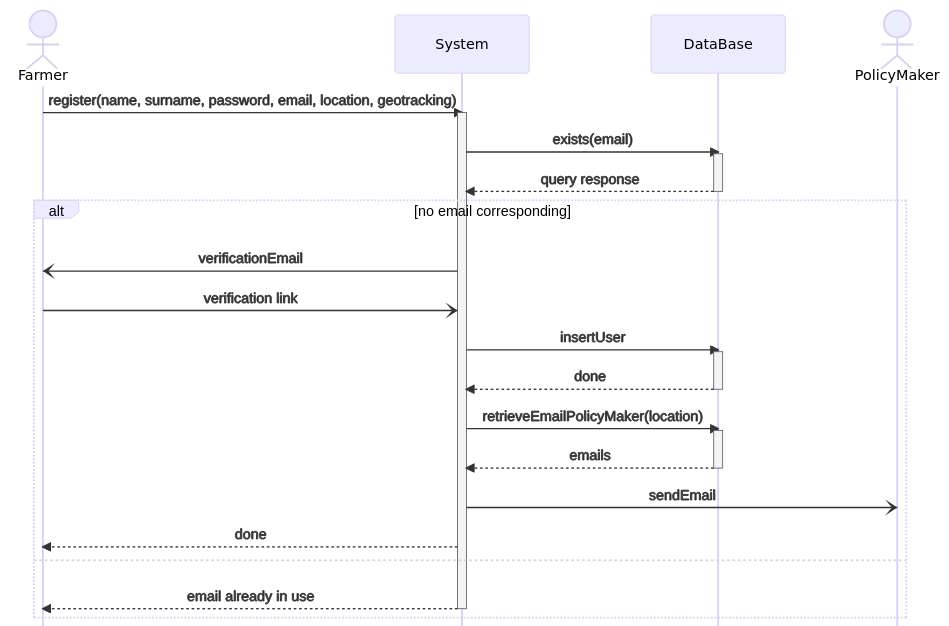
\includegraphics[width=\textwidth]{Images/seq_registration.png}
	
	\caption{\label{fig:seqregistration} Sequence diagram on the registration of a farmer}
	
\end{figure}



\begin{figure}
	
	\centering
	
	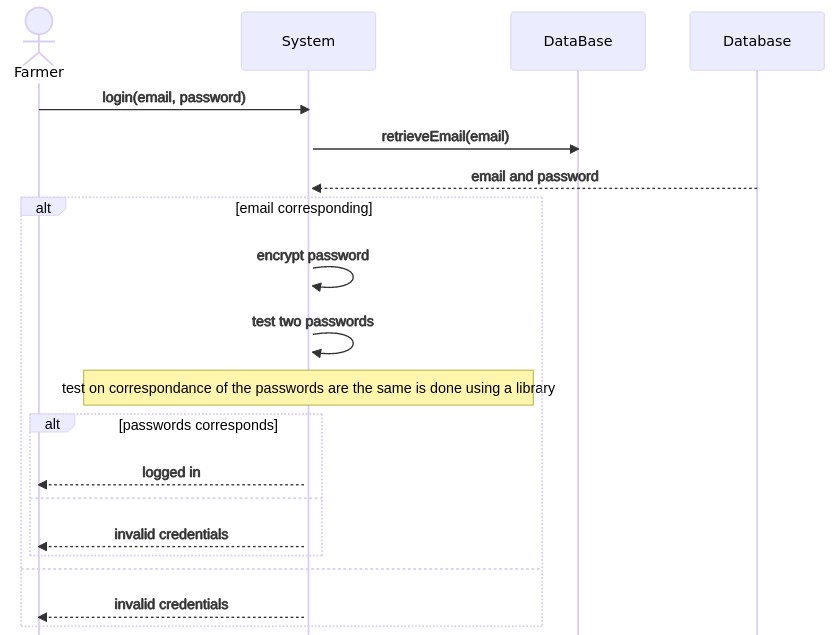
\includegraphics[width=\textwidth]{Images/seq_login.png}
	
	\caption{\label{fig:seqlogin} Sequence diagram on the login of a farmer}
	
\end{figure}



\begin{figure}
	
	\centering
	
	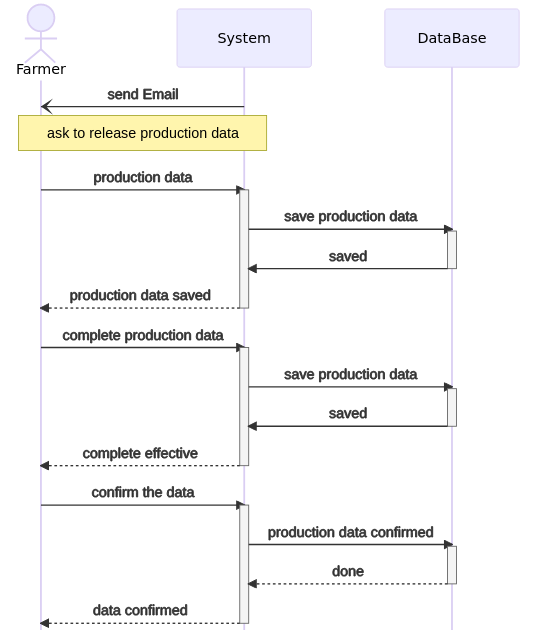
\includegraphics[width=\textwidth]{Images/seq_request_data.png}
	
	\caption{\label{fig:seqrequestdata} Sequence diagram on the request for production data from a farmer point of view}
	
\end{figure}

\begin{figure}
	\centering
	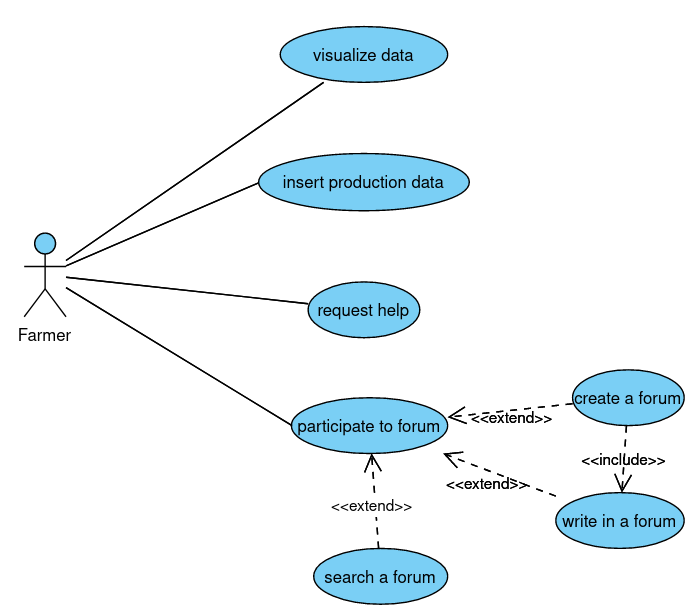
\includegraphics[width=\textwidth]{Images/use-case-farmer.png}
	\caption{\label{fig:usecasefarmer}Use case diagram for logged in farmer}
\end{figure}

\begin{figure}
	\centering
	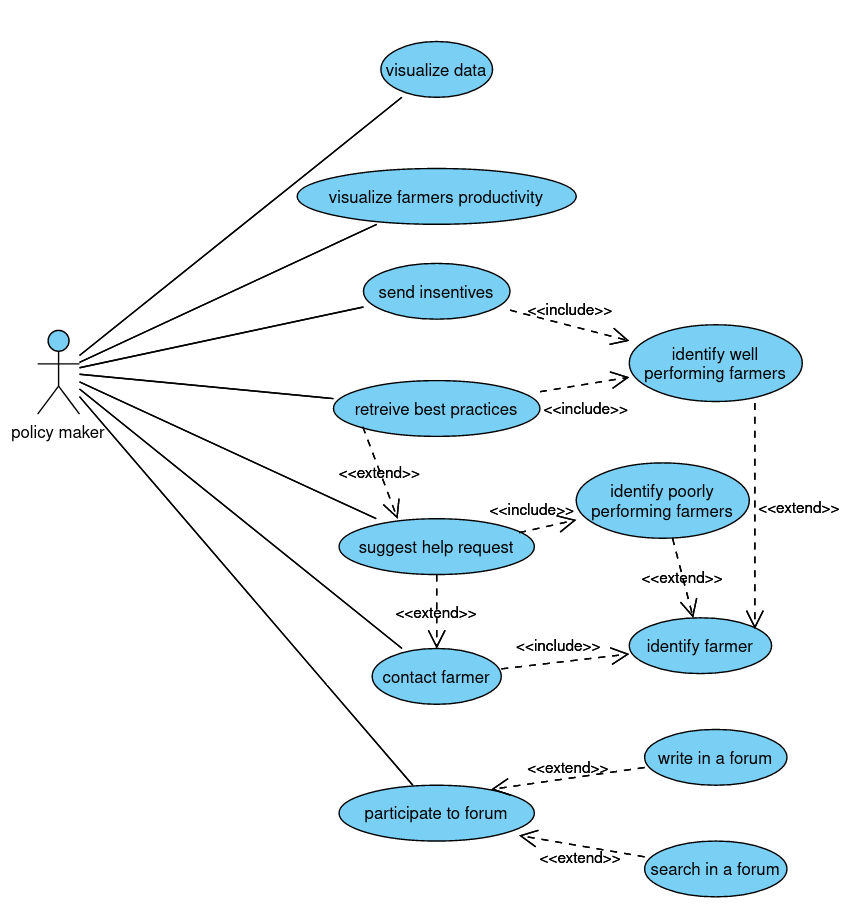
\includegraphics[width=\textwidth]{Images/use-case-policy.png}
	\caption{\label{fig:usecasepolicymakers}Use case diagram for logged in policy makers}
\end{figure}


\begin{figure}
	\centering
	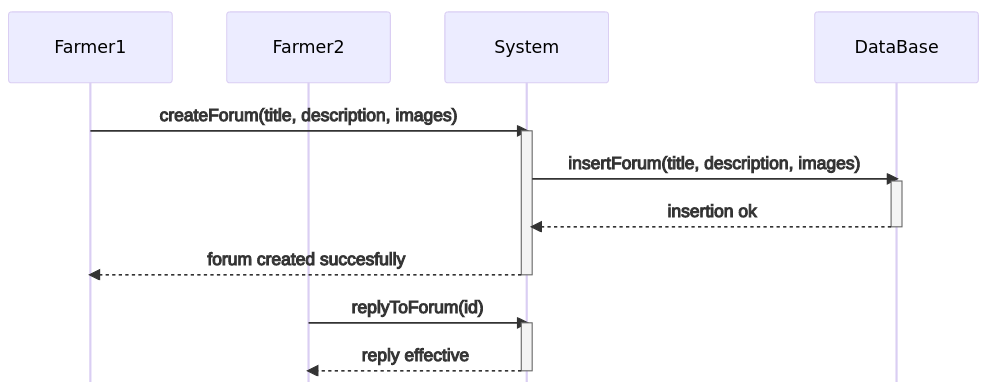
\includegraphics[width=\textwidth]{Images/seq-create-forum.png}
	\caption{\label{fig:seqcreationforum} Sequence diagram on the creation of a forum and the reply by another farmer}
\end{figure}

\begin{figure}
	\centering
	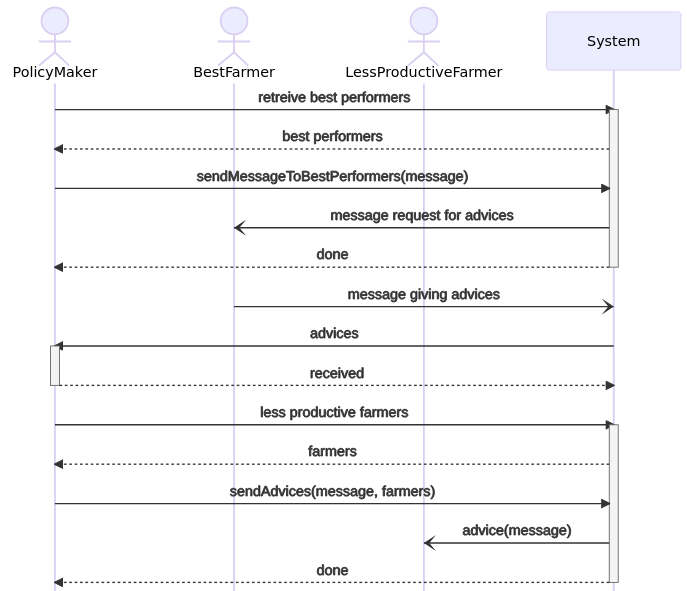
\includegraphics[width=\textwidth]{Images/seq-policy-farmers.png}
	\caption{\label{fig:seqpolicymaker} Sequence diagram showing a policy marker reaching out best performing farmers for advises and send them to less productive farmer}
\end{figure}

\subsection{Performance Requirements}

\subsection{Design Constraints}
\subsubsection{Standards compliance}
\subsubsection{Hardware limitations}
\subsubsection{Any other constraint ??}
Do we keep it ?
\subsection{Software System Attributes}
\subsubsection{Reliability}
\subsubsection{Availability}
\subsubsection{Security}
\subsubsection{Maintainability}
\subsubsection{Portability}
